\chapter{Evaluation}

Die Untersuchung des DELF-Verfahrens lässt sich in zwei wesentliche Abschnitte unterteilen. Zunächst werden in breit angelegten Experimentalreihen unterschiedliche Parameter innerhalb der DELF-Pipeline variiert, um ihren Einfluss auf die Ergebnisse der gelösten Retrievalaufgaben zu quantifizieren. Ziel ist dabei, sowohl ein besseres Verständnis für die Einflüsse einzelner Parameter zu schaffen, wie auch eine optimale Konfiguration für die Lösung von Retrievalaufgaben speziell für historische Bilder zu finden. \\
Im zweiten Abschnitt der Evaluation werden die Entscheidungen des optimierten DELF-Modells qualitativ untersucht, um ein besseres Verständnis für die Entscheidungsfindung des DELF-Prozesses zu erlangen. Insbesondere wird hier DELF mit anderen Retrievalverfahren verglichen, um Schwächen und Stärken des Verfahrens aufzudecken.

\section{Evaluationsdaten}

Zur Bewertung von Retrievalsystemen auf historischen Bildern steht ein eigens erstellter Datensatz zur Verfügung (vgl. Tab. \ref{hist4d_data}). Die 848 zusammengestellten Bilder umfassen historische Abbildungen von sieben Dresdner Sehenswürdigkeiten und entstammen vorwiegend den Archiven der deutschen Fotothek\footnote{\url{https://www.slub-dresden.de/sammlungen/deutsche-fotothek/}, zuletzt besucht am 02.09.20}. Auf Grund der geographischen Nähe einiger Sehenswürdigkeiten sind auf einigen Bildern des Datensatzes mehrere Objekte abgebildet. Bei der Auswertung gelten Bilder für alle Anfragen als korrekte Rückgabe, die mindestens ein Objekt zeigen, welches im betrachteten Bild zu erkennen ist. Bilder die auch als Suchanfrage verwendet werden sind immer genau einer Sehenswürdigkeit zuzuordnen.\\
\begin{table}[h]
\centering

\begin{tabular}{l|c|c|c|c|c|c|c}
\rowcolor[HTML]{C0C0C0} 
Objekt &
  \multicolumn{2}{c|}{\cellcolor[HTML]{C0C0C0}Zwinger} &
  \multicolumn{2}{c|}{\cellcolor[HTML]{C0C0C0}Hofkirche} &
  \multicolumn{2}{c|}{\cellcolor[HTML]{C0C0C0}Frauenkirche} &
  Semperoper \\
Anzahl Objektimpressionen & \multicolumn{2}{c|}{374} & \multicolumn{2}{c|}{216} & \multicolumn{2}{c|}{206} & 89    \\
Anzahl Anfragen           & \multicolumn{2}{c|}{6}   & \multicolumn{2}{c|}{8}   & \multicolumn{2}{c|}{7}   & 7     \\ \hline
\rowcolor[HTML]{C0C0C0} 
Objekt &
  \multicolumn{2}{c|}{\cellcolor[HTML]{C0C0C0}Sophienkirche} &
  \multicolumn{2}{c|}{\cellcolor[HTML]{C0C0C0}Stallhof} &
  \multicolumn{2}{c|}{\cellcolor[HTML]{C0C0C0}Moritzburg} &
  Total \\
Anzahl Objektimpressionen & \multicolumn{2}{c|}{66}  & \multicolumn{2}{c|}{38}  & \multicolumn{2}{c|}{23}  & 1012  \\
Anzahl Anfragen           & \multicolumn{2}{c|}{6}   & \multicolumn{2}{c|}{4}   & \multicolumn{2}{c|}{4}   & 42    \\ \hline
\rowcolor[HTML]{C0C0C0} 
Impressionen pro Bild     & \hspace{2.5mm} 0 \hspace{2.5mm}         & 1           & \hspace{1.1mm} 2 \hspace{1.1mm}           & 3          & \hspace{2mm} 4 \hspace{2mm}           & 5          & Total \\
Anzahl Bilder             & 0          & 730         & 81          & 29         & 7           & 1          & 848  
\end{tabular}%

\caption{Aufbau des historischen Datensatzes}
\label{hist4d_data}
\end{table}
Vorabexperimente haben gezeigt, dass die von DELF durchgeführte Deskriptorselektion nur befriedigende Ergebnisse liefert, wenn die verwendeten Bilder eine Mindestgröße einhalten. Im Selektionsschritt wählt das Attention-Netzwerk eine feste Anzahl an Deskriptoren. Da die Anzahl an extrahierten Deskriptoren je Bild mit der Bildgröße skaliert kann es bei sehr kleinen Bildern passieren, dass das Attention-Netzwerk alle, oder ein Großteil der extrahierten Deskriptoren auswählt. In diesem Fall findet keine bedeutsame Auswahl an Deskriptoren statt und der positive Effekt des Selektionsprozesses geht verloren (siehe Abb. \ref{small_img}).
\begin{figure}[h]
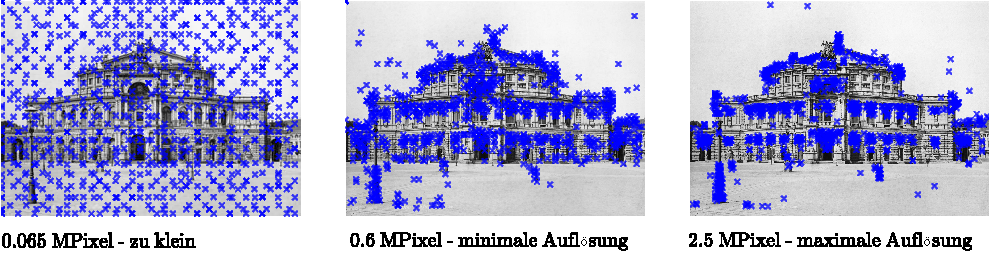
\includegraphics[scale=0.955]{scale_descriptor_selection.pdf}
\caption{Referenzpunkte der ausgewählten Deskriptoren bei unterschiedlicher Eingangsauflösung.}
\label{small_img}
\end{figure}
Auch sehr große Bilder können zu Problemen führen. Da die Bilder während dem Extraktionsprozess in mehreren Skalen betrachtet werden, können bei sehr großen Bildern Speicherproblem auftreten. Aus diesem Grund wird für die Bilder des Datensatzes eine minimale Auflösung von $0.6$MPixel und eine maximale Auflösung von $2.5$MPixel gefordert. Bilder die diese Restriktionen über- bzw. unterschreiten, werden auf die Maximal- bzw. Mindestgröße skaliert.\\
Neben historischen Daten wird das DELF-Verfahren zusätzlich auf dem Oxford5k-Datensatz \cite{oxford5k} getestet (vgl. Tab. \ref{oxford5k_data}). Hierbei handelt es sich um einen häufig verwendeten Benchmarkdatensatz, bestehend aus $5063$ Bildern. Das Bildmaterial entstammt Suchanfragen zu $11$ unterschiedlichen Sehenswürdigkeiten in und um Oxford, an die Fotocommunity Flickr\footnote{\url{https://www.flickr.com/}, zuletzt besucht am 03.09.20}. Häufig finden sich dabei Bilder von Personen oder Aufnahmen von Innenräumen, die keine der gesuchten Sehenswürdigkeiten abbilden. Diese Störbilder können entweder als zusätzliche Herausforderung angesehen oder aber vorab aussortiert werden. In den in dieser Arbeit durchgeführten Experimenten sind diese Störbilder im Datensatz enthalten. 
\begin{table}[h]
\centering
\begin{tabular}{l|c|c|c|c}
\rowcolor[HTML]{C0C0C0} 
Objekt                 & Radcliffe Camera & Christ Church & All Souls   & Magdalen \\
Anzahl Objektimpressionen & 348              & 133           & 111         & 103      \\
Anzahl Anfragen           & 5                & 5             & 5           & 5        \\ \hline
\rowcolor[HTML]{C0C0C0} 
Objekt                & Hertford         & Ashmolean     & Bodleian    & Balliol  \\
Anzahl Objektimpressionen & 61               & 31            & 30          & 18       \\
Anzahl Anfragen           & 5                & 5             & 5           & 5        \\ \hline
\rowcolor[HTML]{C0C0C0} 
Objekt                 & Cornmarket       & Keble         & Pitt Rivers & Total    \\
Anzahl Objektimpressionen & 13               & 11            & 8           & 867      \\
Anzahl Anfragen           & 5                & 5             & 5           & 55       \\ \hline
\rowcolor[HTML]{C0C0C0} 
Impressionen pro Bild     & 0                & 1             & 2           & Total    \\
Anzahl Bilder             & 4218             & 823           & 22          & 5063    
\end{tabular}%
\caption{Aufbau des Oxford5k Datensatzes}
\label{oxford5k_data}
\end{table}

\section{Retrievalmetriken}

Obwohl sich Klassifikations- und Retrievalaufgaben im Kern ähneln, können viele Metriken mit denen Klassifikationssysteme üblicherweise bewertet werden, wie beispielsweise Genauigkeit, nicht verwendet werden, um die Performanz von Retrievalsystemen zu evaluieren. Generell lassen sich aus der Betrachtung einzelner Bildpaare bestehend aus Anfragebild und Bildern des Suchindexes keine Rückschlüsse über die Performanz von Retrievalsystems ziehen.  Grundlage der Bewertung sind stets die gesamten Antworten des Retrievalsystems auf eingehende Suchanfragen. Entscheidend sind hierbei die Rankings, bzw. die Reihenfolgen in der die Bilder des Suchindexes auf die Anfragen zurückgegeben werden. Eine Möglichkeit diese Reihenfolgen zu bewerten ist die Erstellung sogenannter ROC-Kurve (Reciever-Operating-Characteristic)(vgl. Abb. \ref{metric_curve}a). Hierfür wird jeweils eine wachsender Anteil der zurückgegeben Bilder betrachtet und das Verhältnis zwischen Richtig-Positiv-Rate bzw. Recall und Falsch-Positiv-Rate dargestellt. Der Recall gibt an, welcher Anteil an Bildern mit gewünschten Bildinhalt bereits im betrachteten Abschnitt der Rückgabe enthalten war.
\begin{equation}
\text{Recall} = \frac{|\text{Bereits züruckgebene Bilder mit gewünschtem Inhalt}|}{|\text{Im Datensatz enthaltene Bilder mit gewünschtem Inhalt}|}
\end{equation}
Analog beschreibt die Falsch-Positiv-Rate den Anteil der Bilder ohne gewünschten Bildinhalt, der bereits zurückgegeben wurde.
\begin{equation}
\text{Falsch-Positiv-Rate} = \frac{|\text{Bereits züruckgebene Bilder ohne gewünschtem Inhalt}|}{|\text{Im Datensatz enthaltene Bilder ohne gewünschtem Inhalt}|}
\end{equation}
\begin{figure}[h]
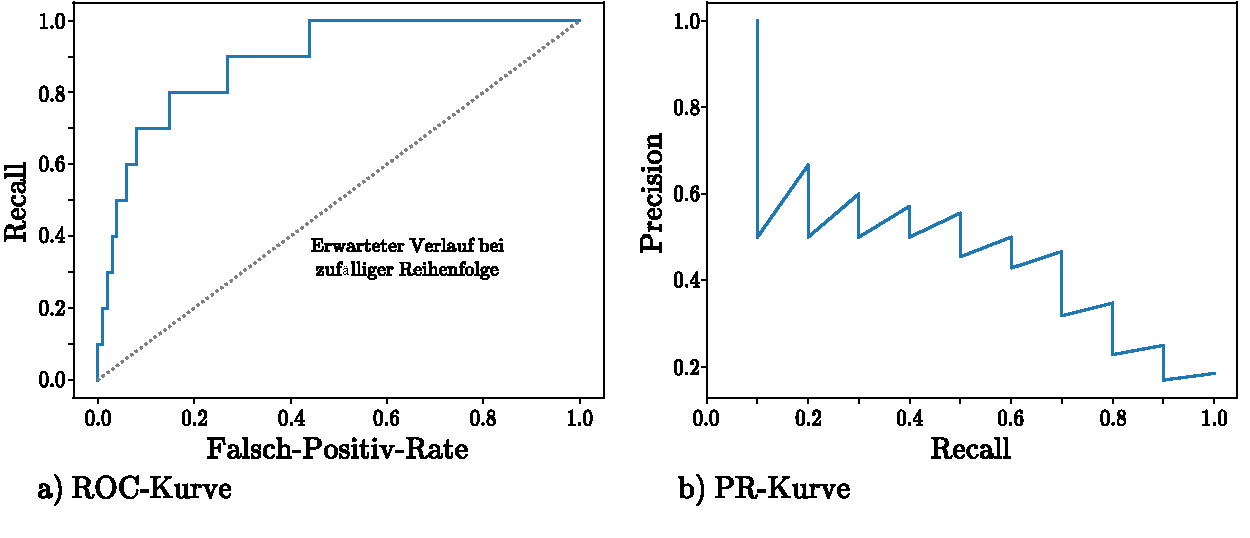
\includegraphics[scale=0.76]{metric_curves.pdf}
\caption{Vergleich von Kurvenmetriken einem Beispielsranking}
\label{metric_curve}
\end{figure}
\\
ROC-Kurven beginnen stets im Ursprung, wo noch keine Bilder zurückgegeben wurden und enden im Punkt $(1,1)$ wo der gesamte Datensatz zurückgegeben wurde. Die Gerade zwischen diesen Punkten bildet den erwarteten Verlauf, wenn das System Bilder in einer zufälligen Reihenfolge zurückgibt. Ein Retrievalsystem hat nur dann einen positiven Effekt für den Nutzer, wenn die ROC-Kurven ihrer Anfrageantworten oberhalb dieser Linie verlaufen. Obwohl ROC-Kurven gut in der Lage sind den Unterschied eines Suchsystems gegenüber einer zufälligen Suche aufzuzeigen, vermitteln sie aus der Perspektive eines tatsächlichen Anwenders oft ein zu positives Bild der Ergebnisse. Das liegt daran, dass der Anteil der Bilder, die für eine Anfrage relevant sind meist um ein vielfaches kleiner ist als der Anteil der irrelevanten Bilder, was an einer ROC-Kurve jedoch nicht ablesbar ist. Angenommen für eine Suchanfrage sind $10\%$ eines durchsuchten Datensatzes tatsächlich relevant und die zur Anfrageantwort erstellte ROC-Kurve zeigt bei einem Recall von $90\%$ eine Falsch-Positiv-Rate von $30\%$. Obwohl der Verlauf der Kurve ein sehr gutes Ergebnis suggeriert, sind für den Nutzer $75\%$ der zurückgegebenen Bilder irrelevant, die er gesehen hat, bevor ein Recall von $90\%$ erreicht wurde. Eine Möglichkeit, die tatsächliche Nutzererfahrung besser abzubilden ist die Erstellung von sogenannten PR-Kurven (Precision-Recall) (vgl. Abb. \ref{metric_curve}b). Hierbei wird die Präzision, also der Anteil der relevanten Bildern in der bisherigen Rückgabe gegen den Recall abgebildet.
\begin{equation}
\text{Precision} = \frac{|\text{Bereits züruckgebene Bilder mit gewünschtem Inhalt}|}{|\text{Bereits züruckgebene Bilder}|}
\end{equation}
So kann direkt abgelesen werden, welchen Anteil an irrelevanten Bildern innerhalb der Rückgabe toleriert werden müssen, um einen bestimmten Anteil der gesuchten Bilder zu finden.
Die vorgestellten Kurvenmetriken eigenen sich gut um einzelne Anfragen an Retrievalsysteme zu analysieren und zu visualisieren. Um Retrievalsysteme in Gänze, auf Basis mehrerer Anfrage zu bewerten und mit anderen Systemen zu vergleichen, bietet es sich an ein kompaktere Metriken zu verwenden. Hierfür wird können die Flächen unterhalb der Metrikkurven betrachtet werden. AUC (Area Under Curve) und AP (Average Percision) beschrieben jeweils die Flächen unterhalb von ROC bzw. PR-Kurven und können so eine Anfrageantwort mit einer einzelnen Zahl bewerten. Auf Grund der besseren Beschreibung des Nutzererlebnisses werden in dieser Arbeit PR-Kurven bzw. AP-Werte zur Auswertung genutzt. Für den Vergleich zwischen unterschiedlichen Retrievalsystemen oder Konfigurationen von DELF werden die AP-Werte von mehreren Anfragen an ein System zu einem Mittelwert (mAP) zusammengefasst. So kann die Performanz eines Retrievalsystems in einer einzelnen Zahl dargestellt werden. 
 

\section{Parameter Analyse}

Ein wesentliches Ziel dieser Arbeit ist es das DELF-Verfahren insbesondere für den Anwendungsfall des Retrievals von historischen Abbildungen zu optimieren. Hierfür werden ein Reihen an Parametern entlang der DELF-Pipeline variiert und ihre Einflüsse, auf die Retrievalergebnisse analysiert.
Die benötigte Rechenleistung zur Durchführung der Experimente wird freundlicherweise vom 
Zentrum für Informationsdienste und Hochleistungsrechnen (ZIH) an der TU Dresden zur Verfügung gestellt. Das verwendete HPC-DA System\footnote{\url{https://tu-dresden.de/zih/hochleistungsrechnen/hpc}, zuletzt besucht am 28.07.20} ermöglicht es viele Experimente parallel und effizient durchzuführen, sodass auch im zeitlich überschaubaren Rahmen dieser Arbeit eine große Anzahl unterschiedlicher Konfigurationen getestet werden können.

\subsection{Hyperparameteroptimierung der Trainingsphasen}\label{hyperparam}
Die ersten Experimentalreihen befassen sich mit den Trainingsphasen des DELF-Verfahrens. Um bei späteren Retrievalversuchen gute Ergebnisse erzielen zu können, benötigt man Modelle die in der Lage sind aussagekräftige Bildrepräsentationen zu erstellen. Für die Experimente zum Modelltraining wird dabei angenommen, dass die Güte, der von einem Modell erzeugten Deskriptoren bzw. der von einem Modell getroffenen Auswahl an Deskriptoren positiv mit der Fähigkeit, der Modelle korreliert die beim Training gestellte Klassifikationsaufgaben zu lösen. Um die Modelle zu bewerten wird daher der Fehler, in Form der Kreuzentropie betrachtet, der auftritt wenn das Modell einen Validierungsdatensatz klassifiziert. Vor Beginn jedes Experiments werden zufällig $20\%$ der Trainingsbilder (siehe Kap. \ref{trainingsdata} auf Seite \pageref{trainingsdata}) für die Validierung ausgewählt. Die Validierungsdaten stehen dem Modell während des Trainingsprozesses nicht zur Verfügung. Daher können sie genutzt werden, um zu überprüfen, ob ein Modell auch auf ungesehenen Daten vergleichbare Ergebnisse erzielt.
\\
Der Erfolg des Trainingsprozesses hängt wesentlich von der zu trainierenden Architektur und der vorhandenen Datenlage ab. Einfluss haben außerdem Parameter, die den Ablauf des Trainingsprozesses beeinflussen. Die Experiments, die in diesem Abschnitt besprochen werden befassen sich mit der Suche nach optimalen Werten für drei dieser sogenannten Hyperparameter. Betrachtet wird die Anzahl der Trainingsepochen, die Lernrate, die bestimmt wie stark Netzwerkparameter in einem Optimierungsschritt angepasst werden, sowie der Faktor $\gamma$ mit dem die Lernrate alle $10$ Epochen multipliziert wird\footnote{Als weiterer Hyperparameter wird weight decay untersucht, allerdings lässt sich hier kein signifikanter Einfluss auf den Validierungsfehler feststellen. Die Ergebnisse hierzu finden sich im Anhang ab Seite \pageref{weight_decay}}. Die übrigen Hyperparameter sind für alle Experimente fest gesetzt. Die Modelle werden mit einer Batchgröße von $8$ trainiert und mittels Stochastic Gradient Decent (kurz SGD \footnote{\url{https://pytorch.org/docs/stable/optim.html\#torch.optim.SGD}, zuletzt besucht am 30.07.20}) optimiert. Für die zu untersuchenden Hyperparameter werden jeweils Wertebereiche definiert. Die Länge des Trainings kann zwischen $10$ und $40$ Epochen dauern. Die initiale Lernrate wird zwischen $0.01$ und $0.001$ gewählt und der $\gamma$-Faktor liegt im Bereich zwischen $1$ und $0.1$.
\\
Um den Suchraum effizient erkunden zu können wird das von Norman Koch entwickelte NNOPT-Tool verwendet, um neue Hyperparameterkonfigurationen zu erstellen und auf dem HPC-System zu testen. Das NNOPT-Tool, das auf dem Hyperopt-Paket \cite{hyperopt} von Bergstra, Yamins und Cox basiert, wählt automatisch Werte für die zu untersuchenden Hyperparameter innerhalb der definierten Wertebereiche aus und startet mit diesen Experimente auf dem Großrechner. Ist ein Experiment abgeschlossen erhält NNOPT zur Bewertung der Konfiguration den erzielten Validierungsfehler. Neue Konfigurationen werden bevorzugt in der Nähe von bereits getesteten Konfigurationen erstellt, die gute Ergebnisse erzielt haben. Dies erlaubt es schneller optimale Hyperparameterwerte zu finden, als mit einer zufälliger Suche.
\\
Für das Fine-Tuning wurden auf diese Art $22$ unterschiedliche Konfigurationen getestet. Es lässt sich beobachten, dass fast alle getesteten Konfigurationen Modell erzeugen, die in der Lage sind die Trainingsaufgabe sehr gut zu lösen. Im Schnitt erzielen die trainierten Modelle eine Klassifikationgenauigkeit von $95.13\%$ auf den Validierungsdaten\footnote{Obwohl zum Vergleich der Konfigurationen der Validierungsfehler berechnet wurde, wird die Modellperformanz im Folgenden über die Validierungsgenauigkeit dargestellt, da diese Metrik intuitiver ist.}, wobei $20$ der $22$ Modelle eine Genauigkeit von über $90\%$ erreichen(vgl. Abb.\ref{finetuning_int_end}b). Da auf Grund der guten Ergebnisse nur wenig Potential für Verbesserung besteht und die beobachtet Varianz der Ergebnisse unterschiedlicher Konfigurationen gering ist, werden keine weiteren Testläufe zur Hyperparameteroptimierung durchgeführt. Es sei jedoch erwähnt, dass sich auf Grund der im Verhältnis zu Größe der Suchraumes geringen Anzahl an Testläufen keine eindeutigen Abhängigkeiten zwischen Hyperparametern und Klassifikationsperformanz ableiten lassen.
\\
Gut beobachten lässt sich der positive Effekt der Nutzung eines vortrainierten Modells zu Initialisierung der Netzwerkparameter. So erreichen alle getesteten Konfigurationen bereits nach der ersten Trainingsepoche eine Validierungsgenauigkeit von über $85\%$ (vgl. Abb.\ref{finetuning_int_end}a). Die initialisierten Parameter müssen nur noch geringfügig angepasst werden, um die neue Trainingsaufgabe zu lösen, weshalb die Modelle von Beginn an gute Ergebnisse erzielen. 
\\
\begin{figure}[h]
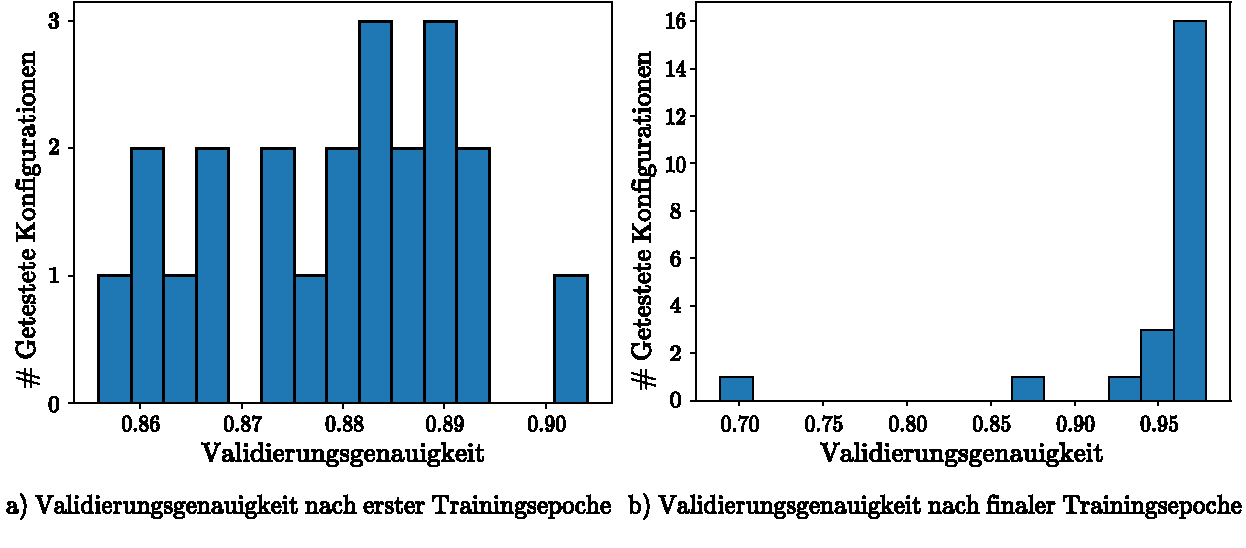
\includegraphics[scale=0.750]{NNOPT/init_and_end_perf_finetuning.pdf}
\caption{Erreichte Klassifikationsgenaugikeit nach der ersten bzw. letzten Epoche des Fine-Tunings, der getesteten Konfigurationen}
\label{finetuning_int_end}
\end{figure}
\\
Betrachtet man die Ergebnisse der Testläufe in Kombination mit den dazugehörigen Hyperparametern (siehe Abb.\ref{finetuning_all}), so scheint die Anzahl an Trainingsepochen keinen signifikanten Einfluss auf die erzielte Validierungsgenauigkeit zu haben. Dies deckt sich mit der Annahme, dass sich Netzwerkparameter mittles Fine-Tuning in wenigen Epochen optimieren lassen. Betrachtet man den Trainingsverlauf des Fine-Tunings (vgl. Abb. \ref{finetuning_lr_gamma_verlauf}), so stellt man fest, das für die meisten Konfigurationen nach $10-15$ Epochen keine großen Verbesserungen mehr im Hinblick auf die Validierungsgenauigkeit erzielt werden.  
\begin{figure}[h]
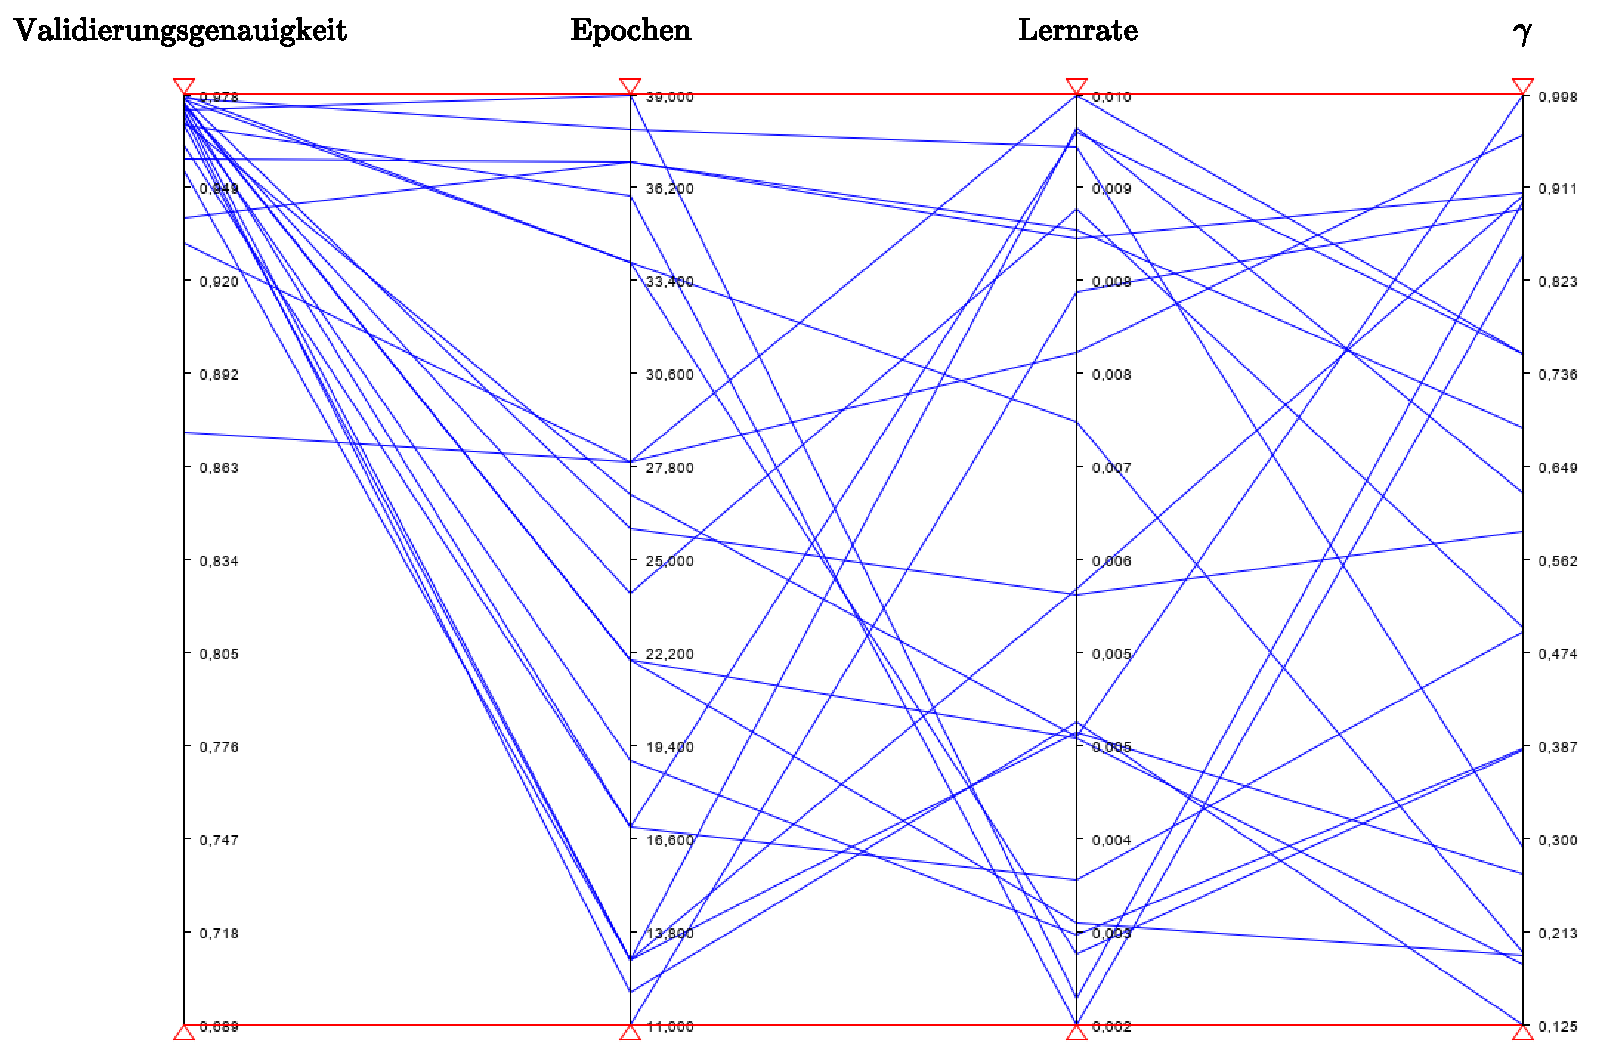
\includegraphics[scale=0.58]{NNOPT/finetuning_all.pdf}
\caption{Parallele Darstellung der getesteten Konfigurationen des Fine-Tunings. Jede Linie repräsentiert einen Konfiguration und die von ihr erzielte Validierungsgenauigkeit.}
\label{finetuning_all}
\end{figure}
\\
Beleuchtet man die in den getesteten Konfigurationen genutzten Lernraten, so stellt sich heraus, dass alle Testläufe mit einer Lernrate unter $0.005$ eine sehr gute Validierungsgenauigkeit erreichen. Werden höhere Lernraten genutzt, so unterscheiden sich die erzielten Ergebnisse deutlich stärker. Bezieht man die dazugehörigen $\gamma$-Faktoren mit ein, sieht man, dass Konfigurationen mit hoher Lernrate, aber niedrigem $\gamma$-Faktor, also mit starker Reduktion der Lernrate während des Trainingsverlaufes, ebenfalls sehr gute Ergebnisse erzielen. Läufe mit hoher Lernrate, sowie hohem $\gamma$-Faktor schneiden dagegen eher schlechter ab (Siehe Abb. \ref{finetuning_lr_gamma}). Analysiert man die Trainingsverläufe der unterschiedlichen Konfigurationen (Siehe Abb.\ref{finetuning_lr_gamma_verlauf}), findet sich eine mögliche Erklärung für diese Verhalten. Bei niedriger Lernrate nähert sich die Validierungsgenauigkeit ohne starke Einbrüche einem Maximum an. Ist die Lernrate hoch fluktuiert die Validierungsgenauigkeit jedoch stark. Dies weist darauf hin, dass die Modelle nicht in der Lage sind ein stabiles Optimum für ihre Parameter zu finden. Hohe Lernraten können dazu führen, dass Parameter bei Optimierungsschritten zu stark verändert werden und so ihr Optimum immer wieder überspringen. Nach Abschluss der ersten $10$ Epochen wird die Lernrate mit dem $\gamma$-Faktor multipliziert. Für Läufe mit hoher initialer Lernrate und niedrigem $\gamma$-Faktor lässt ab diesem Punkt ein gleichmäßigerer Lernprozess beobachten. 
\begin{figure}[h]
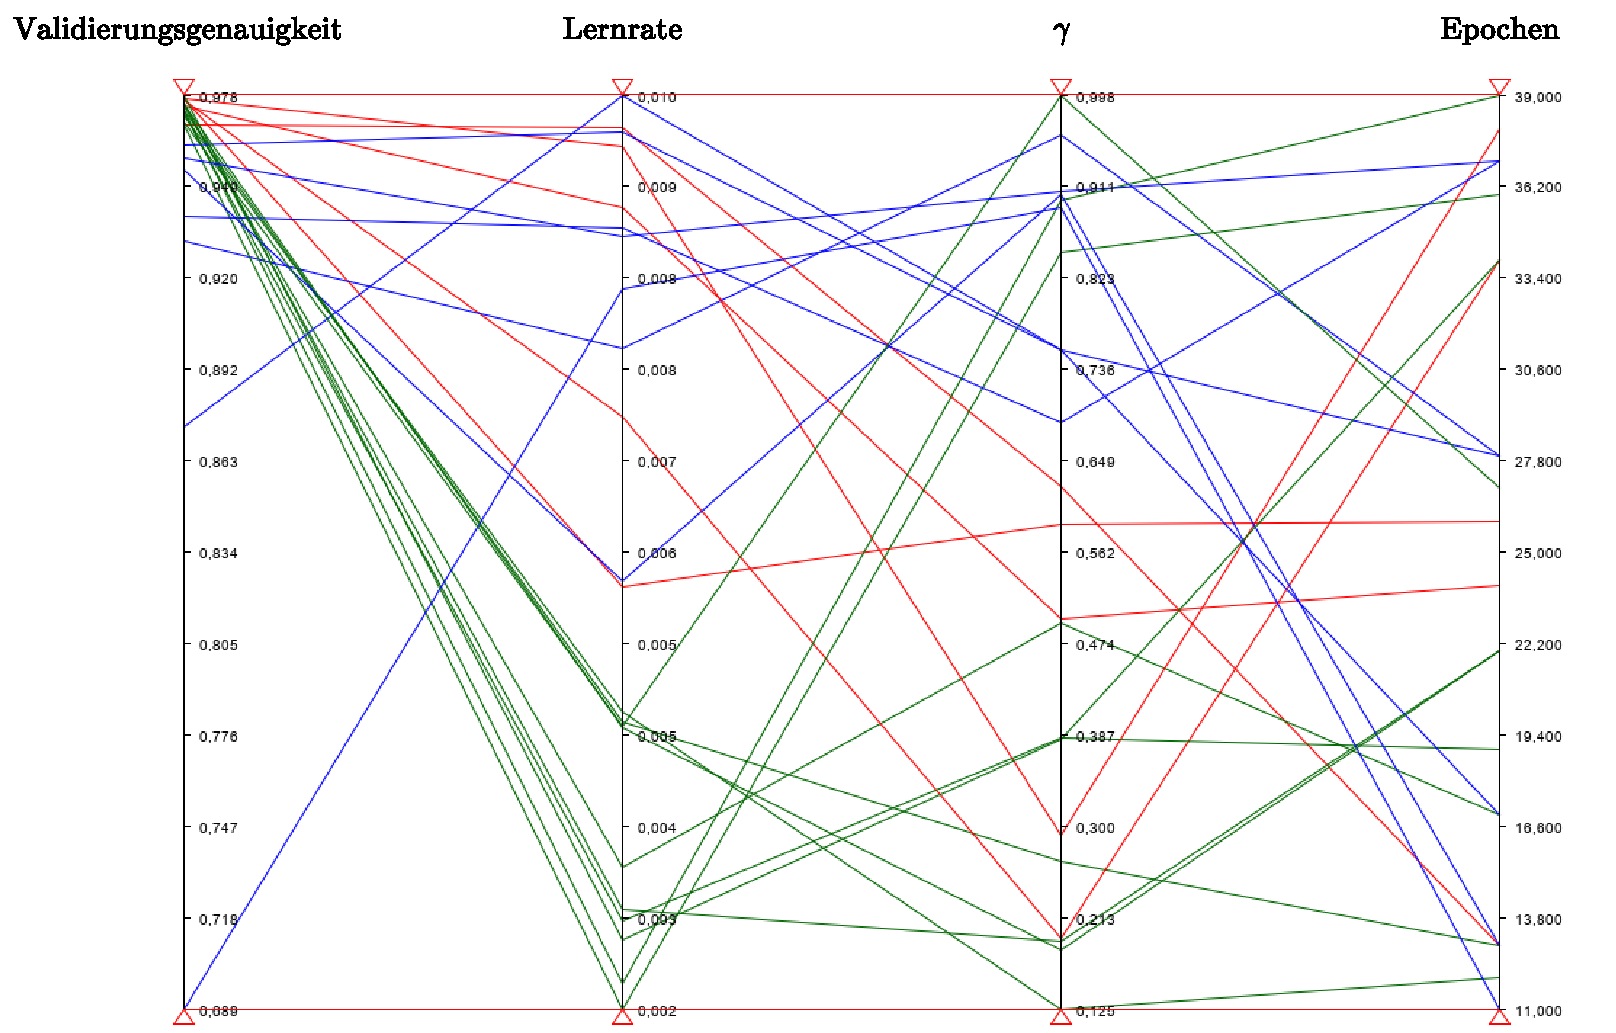
\includegraphics[scale=0.58]{NNOPT/finetuning_lr_gamma.pdf}
\caption{Betrachtung der genutzten Lernraten und $\gamma$-Faktoren. Grün: Konfigurationen mit niedriger Lernrate $(<0.005)$, Rot: Hohe Lernrate und niedriges $\gamma$ $(<0.65)$, Blau: Hohe Lernrate und hohes $\gamma$}
\label{finetuning_lr_gamma}

\centering
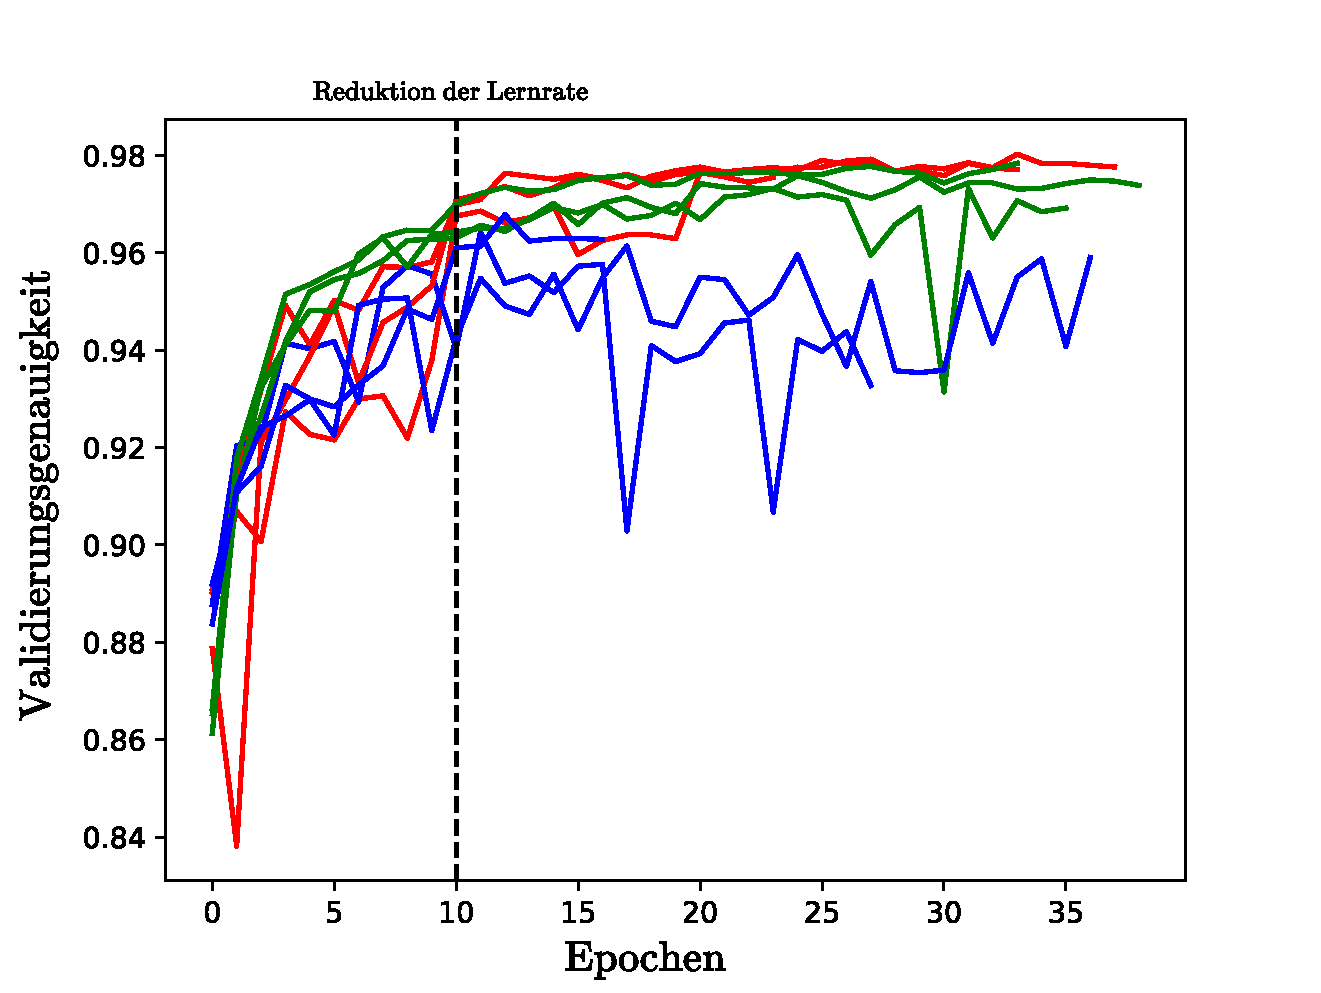
\includegraphics[scale=0.6]{NNOPT/finetuning_lr_gamma_verlauf.pdf}
\caption{Trainingsverlauf der Fine-Tunings, bei unterschiedlicher Lernrate und $\gamma$. Farbgebung analog zu Abb.\ref{finetuning_lr_gamma}}
\label{finetuning_lr_gamma_verlauf}
\end{figure}
\clearpage
Die Konfiguration mit dem besten Trainingsergebnis schreibt eine Trainingsdauer von $22$ Epoche, bei einer initialen Lernrate von $0.0032$ und einem $\gamma$-Faktor von $0.19$ vor und erzielt nach der letzten Epoche eine Validierungsgenauigkeit von $97.6\%$.
\\
Das dabei trainierte Modell ist der Ausgangspunkt für die Hyperparameteroptimierung des Attention-Trainings. Analog wie in den Experimenten zum Fine-Tuning werden mit Hilfe von NNOPT $60$ unterschiedliche Konfigurationen für das Attention-Training getestet. Obwohl das Modell für das Attention-Training durch Entfernung des vierten ResNet-Blocks deutlich verkleinert wird und die Ausgaben des ResNets unter Verwendung des gewichteten Sum-Poolings (vgl. Abb.\ref{attention} auf Seite \pageref{attention}) sehr restriktiv genutzt werden, sind die Attention-Modelle in fast allen untersuchten Konfigurationen in der Lage die Klassifikationsaufgaben weiterhin sehr gut zu Lösen. So werden in $59$ der $60$ untersuchten Konfigurationen eine abschließende Validierungsgenauigkeit von über $89\%$ erreicht (siehe Abb.\ref{attention_int_end}b). Die durchschnittliche Validierungsgenauigkeit nach der letzten Trainingsepoche beträgt $91.3\%$, was einer durchschnittlichen Verschlechterung von $6.3\%$ gegenüber dem verwendeten fine-getunten ResNet-Modell entspricht. Im Kontrast zum Fine-Tuning variiert die gemessene Validierungsgenauigkeit nach der ersten Trainingsepoche der Attention-Trainings deutlich stärker und ist allgemein niedriger (vgl. Abb.\ref{attention_int_end}a). Da die Parameter der zu optimierenden Attention-Einheit nicht vortrainiert sind und daher zufällig initialisiert werden sind größere Unterschiede und schlechter Ergebnisse zu Beginn des Trainings, sowie eine längere benötigte Trainingsdauer zu erwarten.
\begin{figure}[h]
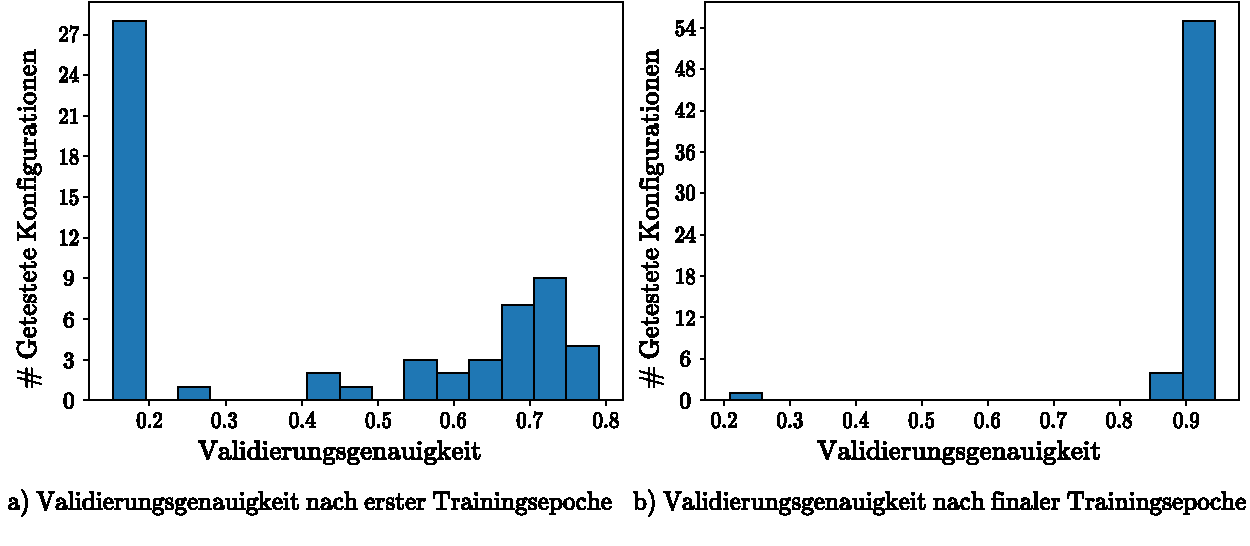
\includegraphics[scale=0.75]{NNOPT/init_and_end_perf_attention.pdf}
\caption{Erreichte Klassifikationsgenaugikeit nach der ersten bzw. letzten Epoche des Attention-Trainings, der getesteten Konfigurationen}
\label{attention_int_end}
\end{figure}
\\
Betrachtet man die genutzte Anzahl an Trainingsepochen in Kombination mit der erreichten Validierungsgenauigkeit(siehe Abb.\ref{attention_epochs}), bestätigt sich diese Annahme. Konfigurationen mit einer Trainingsdauer unter $20$ Epochen erzielen in unseren Experimente durchschnittlich eine geringere Validierungsgenauigkeit. Ab mehr als $20$ Epochen schwächt sich der positive Effekt einer längeren Trainingsdauer jedoch deutlich ab.
\\
\begin{figure}[h]
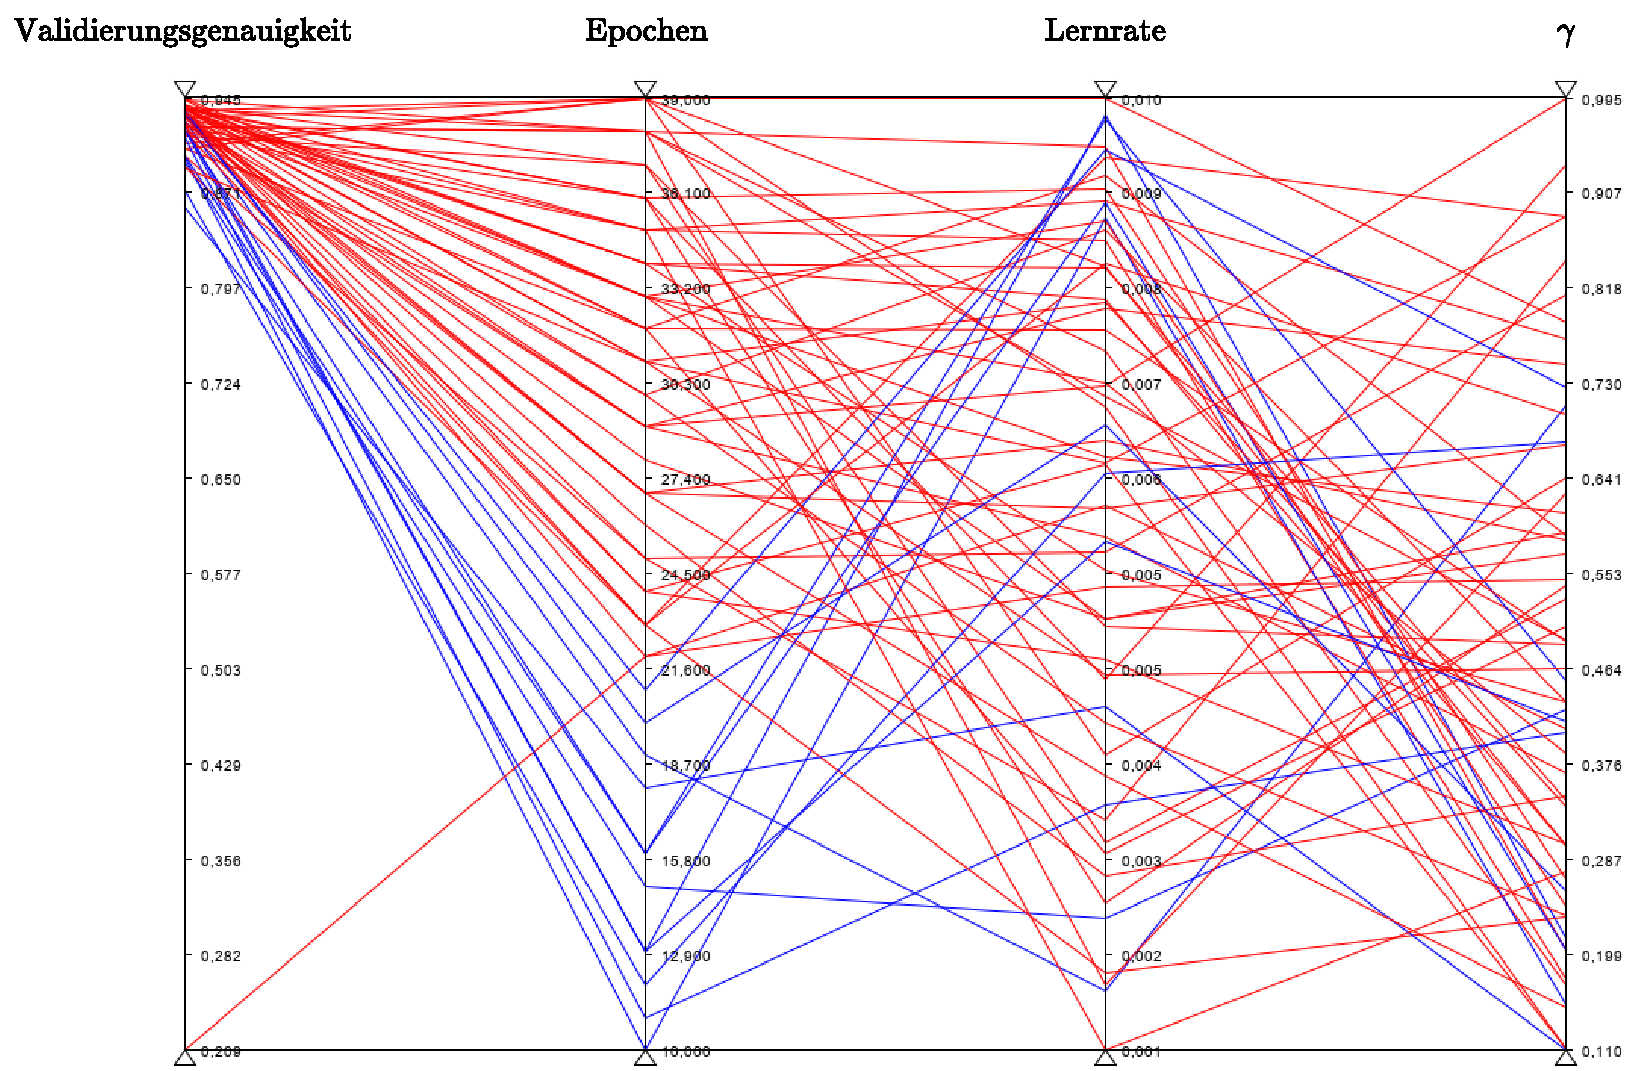
\includegraphics[scale=0.58]{NNOPT/attention_epochs.pdf}
\caption{Betrachtung der gewählten Trainingsdauer. Rot: Über $20$ Epochen, Blau: $20$ oder weniger Epochen}
\label{attention_epochs}
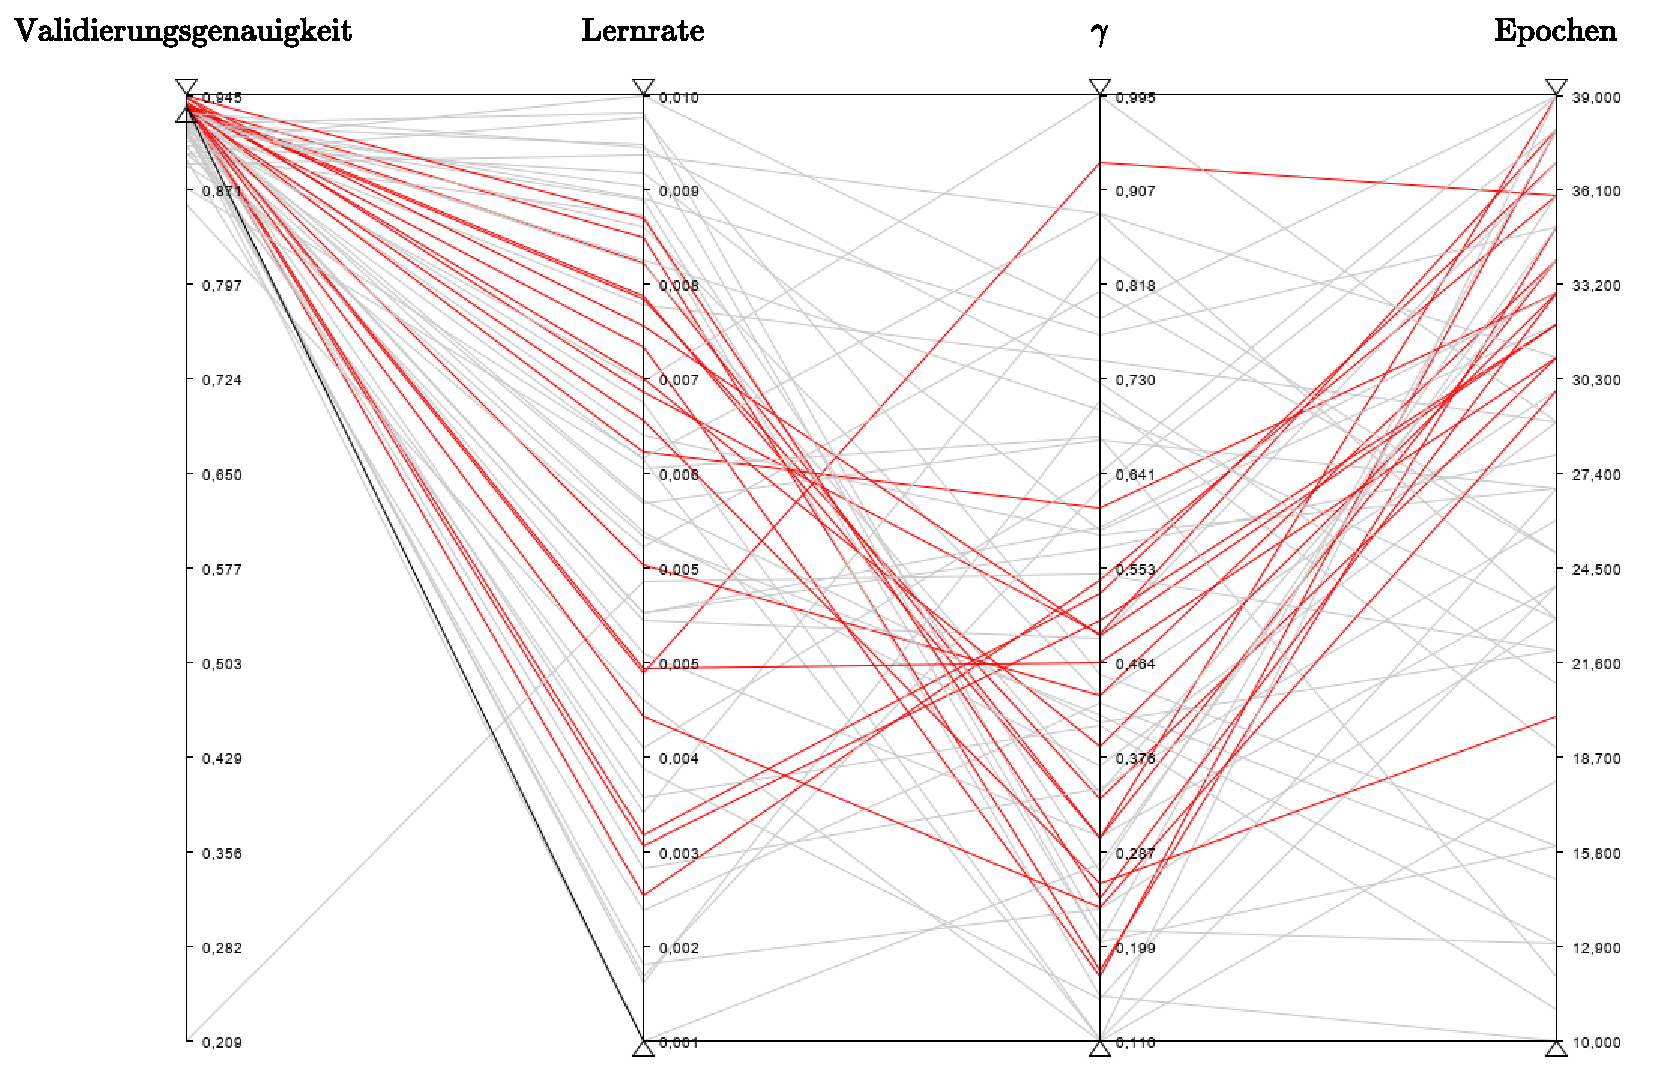
\includegraphics[scale=0.58]{NNOPT/attention_top_runs.pdf}
\caption{Darstellung der Validierungsgenauigkeit nach Trainingsende. Rot: Läufe mit Validierungsgenauigkeit $\geq 93.5\%$, Grau: Läufe mit niedrigerer Validerungsgenauigkeit}
\label{attention_top}
\end{figure}
\clearpage
Für Lernrate und $\gamma$-Faktor lassen sich nur schwer Tendenzen erkennen. Über den gesamten Suchraum dieser Parameter lassen sich sowohl Konfigurationen mit hoher, sowie Konfigurationen mit weniger hoher Validierungsgenauigkeiten erreichen finden. Die Konfigurationen, welche die höchsten Validierungsgenauigkeiten erreichen (Siehe Abb.\ref{attention_top}) nutzen jedoch alle eine Lernrate im Bereich zwischen $0.0025$ und $0.009$. Die $\gamma$-Faktoren dieser Konfigurationen liegen meist unter $0.55$ und die Trainingsdauer über $30$ Epochen.
Die beste gefundene Konfiguration erzielt eine Validierungsgenauigkeit von $94.5\%$ und nutzt dabei eine Lernrate von $0.0078$ einen $\gamma$-Faktor von $0.49$ und eine Trainingslänge von $32$ Epochen. 
Mit Hilfe der ermittelten Hyperparameterwerte der besten gefundenen Konfigurationen für Fine-Tuning und Attention-Training werden $6$ neue Modelle Trainiert, die in den Retrievalexperimenten zur Extraktion der Deskriptoren genutzt werden. Die Trainingsverläufe dieser Modelle sind in Abb.\ref{optimized_runs} dargestellt.
\begin{figure}[h]
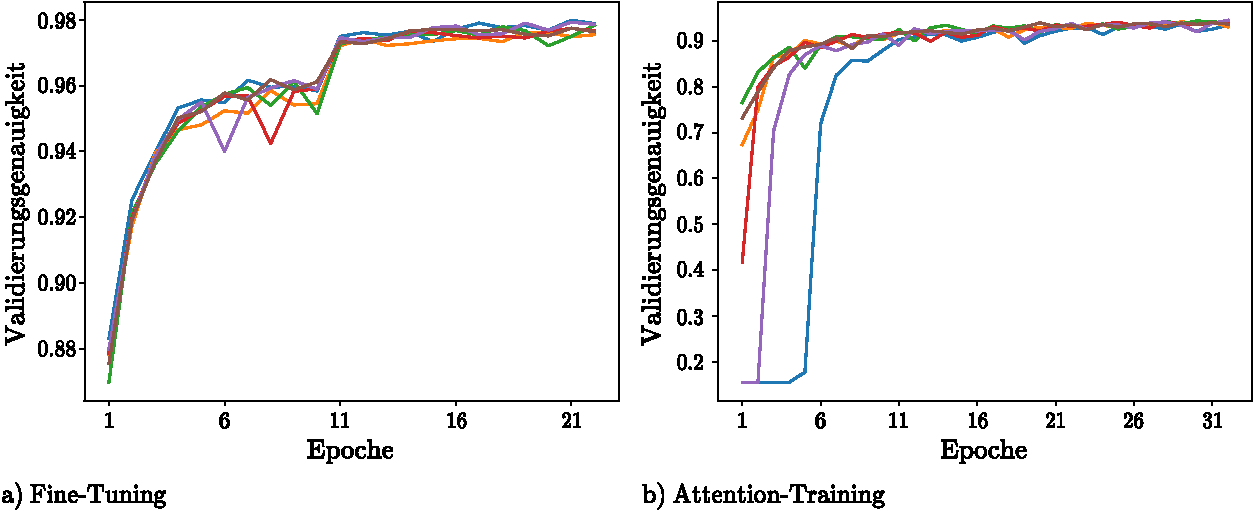
\includegraphics[scale=0.75]{NNOPT/6_model_verlauf}
\caption{Trainingsverläufe mit optimierten Hyperparametern. Gleichefarbige Linen gehören zu gemeinsamen Trainingsläufen.}
\label{optimized_runs}
\end{figure}


 